\subsection{Maßzahlen}
\small\textit{verfasst von Florian Roth}
\normalsize
\\ Im Anschluss an diese Arbeit gilt es zu untersuchen, in wie fern die aufgenommenen Signale geeignet sind um mittels Netzwerkcodierung und Compressed Sensing unter Einsparung von Datenverkehr versendet werden können. 
\\ Um das für eine große Anzahl an Signalen überhaupt möglich zu machen, ist es erforderlich die untersuchten Signale anhand von  bestimmten Eigenschaften zu klassifizieren. Damit ein einfacher Vergleich mehrerer Signale schnell möglich ist, bietet es sich an diese Eigenschaften als Zahlenwert auszudrücken. 
\\ Die beschriebenen Eigenschaften sind entweder physikalischer Natur oder versuchen die Form der Kreuzkorrelation zu charakterisieren. Dabei wurde darauf geachtet, wenn möglich normierte Größen zu verwenden um die Vergleichbarkeit zwischen Signalen unterschiedlicher Abtastrate und Zeitdauer aufrecht zu erhalten. 
\\ Beim Entwerfen solcher Maßzahlen besteht die Schwierigkeit darin, möglichst viel aussagekräftige Information dahingehend zu vereinfachen, dass eine Überführung in eine Zahl überhaupt möglich ist. Gleichzeitig darf durch die Vereinfachung nicht die Aussagefähigkeit der Maßzahl zerstört werden, also die Möglichkeit auf eine Eigenschaft des Signals anhand des Zahlenwertes zurück zu schließen. Aufgrund dieser Anforderungen sind im Verlauf dieser Arbeit mehrere Maßzahlen entstanden, von denen einige im weiteren Prozess wieder verworfen wurden. 
\\Die Bedeutung und Berechnung der finalen Maßzahlen wird hier kurz vorgestellt. 
\subsubsection{ripple}
Die Maßzahl \textit{ripple} trifft eine Aussage über die Energieverteilung im Signal. Zur Berechnung wird die Energie, die die obersten fünf Perzentile der berechneten Werte enthalten, ins Verhältnis zur Gesamtenergie gesetzt. 
\begin{align*}
ripple = \frac{\sum_{\text{der obersten 5 Perzentile}}x_{i}^2}{\sum_{i=1}^{N}x_{i}^2}
\end{align*}
\textit{ripple} kann Werte zwischen 0 und 1 annehmen, wobei $ripple = 0$ bedeutet, dass es sich um eine konstante Funktion handelt, während $ripple = 1$ auf einen einzelnen Impuls schließen lässt.
\subsubsection{sigma}
Ziel war es eine Maßzahl zu finden, die eine Aussage über die Verteilung der größten Werte der Kreuzkorrelation liefert. In einer ersten Version des Programmes wurde die in Octave intigrierte Funktion \textit{xcorr} verwendet, die zero-padding nutzt, wenn sie die Signale im Zeitbereich zueinander verschiebt. Dadurch fiel die KKF zu den Seiten schnell ab und die Hüllkurve erinnerte stark an eine Glockenkurve. Ein Maß für die ,,Breite'' einer Glockenkurve stellt das \textit{sigma} im Exponenten der $e$-Funktion dar. 
\\Auch nach dem Umstellen auf eine andere KKF-Berechnung, bei der durch periodisches Aneinandersetzen der Signale kein Abfall auf Null zu den Rändern stattfindet, konnte in einem Großteil der Korrelationshüllkurven weiterhin eine Glockenkurvenform vorgefunden werden, allerdings nun mit Gleichanteil. Um die gewünschte Maßzahl \textit{sigma} aus den numerisch vorliegenden Werten zu erhalten, muss ein mathematischer Ausdruck für die Hüllkurve gefunden werden. Die Hülllkurve \textit{envelope} wiederum erhält man durch Amplituden-Demodulation der KKF. Dabei wird das Signal gleichgerichtet und auf ein Tiefpassfilter gegeben. Der Filter wird in dieser Arbeit im Frequenzbereich realisiert mit einer von der zeitlichen Länge des Signals $t_{Signal}$ abhängigen Grenzfrequenz $f_{c} = \frac{20}{t_{Signal}}$. Bei dem Zahlenwert $20$ handelt es sich um einen experimentell bestimmten Wert. 
\begin{align*}
envelope = IDFT\lbrace DFT\lbrace|\psi_{\text{XY}}(n)|\rbrace\cdot\text{H}_{\text{TP}}\rbrace
\end{align*}
Für die Hüllkurve \textit{envelope} wird nun mittels Methode der kleinsten Quadrate eine Regressionsrechnung auf die vermutete Glockenkurvenfunktion vorgenommen. Die Funktionsvorschrift lautet dabei
\begin{align*}
y = a\cdot e^{-\frac{(x-\mu)^2}{2\sigma^2}}+b
\end{align*}
Mit den zu bestimmenden Konstanten $a$, $b$, $\mu$ und $\sigma$. Mit dem erhaltenen Wert für $\sigma$ lässt sich keine Aussage über den Anteil der Fläche der Hüllkurve in den Grenzen $\mu-\sigma$ bis $\mu+\sigma$ treffen. Das liegt an dem Gleichanteil und keiner Verknüpfung mit der Amplitude $a$ wie bei der Gauss'schen Glockenkurve. Sehr wohl stellt $\sigma$ allerdings ein Maß für die Breite des peaks rund um den Nullpunkt der Korrelation dar. Die Angabe erfolgt in Sekunden. 
\begin{figure}[ht!]
\centering
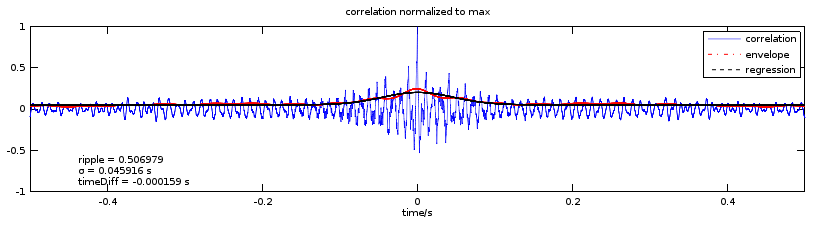
\includegraphics[width=10cm, keepaspectratio=true]{img/lucas_von_flur_in_bad_m_(4s)+1s.png}
\caption{Kreuzkorrelation mit Amplituden-Demodulation und Regression}
\label{AM-Demodulation}
\end{figure}
\subsubsection{timeDiff}
Der Parameter \textit{timeDiff} gibt den zeitlichen Versatz der Stereokanäle zueinander wieder. Dazu wird der Indexwert $i$ des Maximums der Kreuzkorrelation bestimmt und anhand der Samplingrate $r$ die Zeitdifferenz zum Nullpunkt ($\tau = 0$) berechnet.
\begin{align*}
\Delta t = \frac{\Delta i}{r}
\end{align*}
\subsubsection{exp und area}
Da die Regression auf eine Glockenkurve nicht für alle Signale sinnvoll ist, war eine Maßzahl gefordert, die zumindest den Abfall der Gesamtheit aller Amplituden angibt. Dazu wurden die diskreten Werte der Korrelation betragsmäßig absteigend geordnet. Anschließend wurde wieder eine Regressionsrechnung mit Hilfe der Methode der kleinsten Quadrate angewandt. Dabei handelt es sich nun um eine einfache abfallende e-Funktion
\begin{align*}
y = e^{-c \cdot x}
\end{align*}
wobei der ausgegebene Parameter \textit{exp} der ermittelten Konstante $c$ entspricht, normiert auf die Länge des Signals. Bei Vergleich der Regressionskurve mit der ursprünglichen Funktion fällt auf, dass diese nur schlecht angenähert wird. Auf ein modifizieren der Funktion, beispielsweise durch Addition eines Gleichanteils, wird jedoch verzichtet, da die Verrechnung der zusätzlichen Parameter zu einer aussagekräftigen Maßzahl nicht glückte. Ein Maß für den geforderten Abfall stellt auch die einfache e-Funktion dar. 
\\Um einen alternativen Parameter zu bestimmen wird die Fläche unter der Kurve berechnet und auf die Länge des Signals normiert. 
\begin{align*}
area = \frac{1}{N_{\text{samples}}} \sum_{n=1}^{N_{\text{samples}}} |\psi_{\text{XY}}(n)|
\end{align*}
Eine Normierung auf den Maximalwert erfolgt schon beim Berechnen der Kreuzkorrelation. Dadurch kann \textit{area} nur Werte zwischen $0$ und $1$ annehmen. Je kleiner \textit{area}, desto steiler fallen die Amplituden ab. 
\\Trotz der erfolgreich ermittelten Maßzahl \textit{area}, berechnet das Programm weiterhin den Parameter \textit{exp}, denn dieser lässt sich leicht modifizieren und kann somit noch an Aussagekraft hinzu gewinnen. 
\begin{figure}[ht!]
\centering
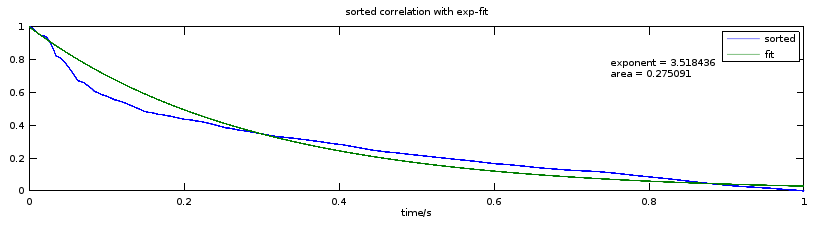
\includegraphics[width=10cm, keepaspectratio=true]{img/trefftz_wiese_m_8(s)+1s_exp.PNG}
\caption{sortierte Kreuzkorrelation mit Regression}
\label{exp-Regression}
\end{figure}
